\chapter{Especificação de Requisitos do Sistema}\label{chap:especificacao-requisitos-sistema}
Neste capítulo, serão abordados os requisitos do sistema encontrados, os pontos levantados nas diversas reuniões e os requisitos funcionais e não funcionais encontrados.

\section{Modelagem do Processo}
No capítulo \ref{chap:aspectos-conceituais}, mostrou-se a importância da modelagem de processos para entender como funciona o processo onde o sistema será inserido. Para isso, o processo das duas disciplinas foi modelado usando BPMN, por meio de conversas realizadas no início do ano.

A primeira reunião de entendimento do processo ocorreu dia 12/03, com a participação dos coordenadores João Batista e Paulo Cugnasca, além do professor Fábio Levy. Nesta reunião, ocorreu o entendimento geral do sistema, as expectativas do projeto e uma abordagem do processo das duas disciplinas.

Com base nessa reunião, foram modelados quatro diagramas principais, cada um abordando uma etapa do processo: TCC1, TCC2 sem as avaliações finais, os eventos de feira e banca e, por fim, a parte de recuperação. Os diagramas se encontram no anexo \ref{chap:bpmn-appendix}, mas a figura \ref{fig:bpmn-geral} aponta o processo de uma maneira geral, com os problemas essenciais representados no diagrama.

O processo consiste em duas disciplinas, com entregas parciais no decorrer de cada uma delas, sendo a primeira responsável por gerar a especificação do trabalho e a segunda pela elaboração da monografia e a implementação do projeto. Em especial, a segunda disciplina possui dois eventos complementares: a feira prática e a banca teórica, com uma premiação dos melhores projetos do ano, compondo o processo completo das disciplinas.

Nas disciplinas de TCC em geral, o problema maior está no envolvimento do orientador com o grupo de trabalho, muitas vezes problemático por falta de comunicação do grupo com o orientador. Além disso, as avaliações são feitas sempre pela visão da coordenação sobre o trabalho, que leva em conta \textit{feedbacks} do orientador, realizados informalmente.

Já nos eventos especiais de avaliação na segunda disciplina, as avaliações ocorrem com formulários em papel, recolhidos após cada evento. Ao final dos eventos, as notas precisam ser calculadas com urgência, por causa da premiação, o que gera transtorno pelo curto prazo e pela chance de falha (formulários perdidos, incompletos, entre outros).

Com base na modelagem do processo completo e com os problemas básicos levantados, ocorreu outra reunião no dia 4/4, para revisar os diagramas que representam o processo das duas disciplinas. Com base no processo revisado, estabeleceu-se a visão, que serve de base para a modelagem em casos de uso, explicada na próxima seção.

\begin{figure}[!htpb]
    \centering
    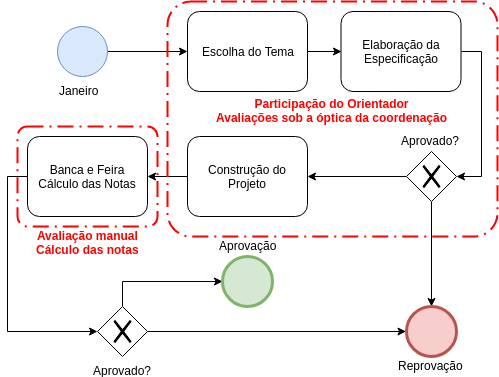
\includegraphics[scale=0.6]{imagens/bpmn_geral.png}
    \caption{Modelagem BPMN do processo geral, com os problemas apontados}
    \label{fig:bpmn-geral}
\end{figure}

\section{Visão do Sistema}
De acordo com o capítulo \ref{chap:aspectos-conceituais}, o documento visão é responsável por unificar o entendimento do sistema para os \textit{stakeholders}.

\subsection{Descrição do Problema}
Os problemas estão na descentralização do processo, com os orientadores participando por intermédio de seus orientados, além da parte manual de construção de eventos e de avaliações das bancas. O impacto direto é na demora e esforço para calcular notas, dificuldade de integração entre envolvidos (orientador, alunos e coordenação). Para resolver o problema, o sistema deve automatizar o processo e integrar os envolvidos ao longo das disciplinas.

\begin{table}[!htb]
    \centering
    \caption{Sentença básica de posição do produto}
    \label{sentenca-posicao}
    \resizebox{480pt}{!}{\begin{tabular}{|l|l|lll}
        \cline{1-2}
        Para            & alunos, orientadores, coordenadores e técnicos                                                                  &  &  &  \\ \cline{1-2}
        Que             & cursam ou estão envolvidos diretamente                                                            &  &  &  \\ \cline{1-2}
        O sistema       & de gerenciamento dos TCC's                                                                                      &  &  &  \\ \cline{1-2}
        Que             & armazena os TCC's anteriores e gerencia o TCC atual, realizando avaliação e controlando entregas                                                             &  &  &  \\ \cline{1-2}
        Ao contrário do & processo semi-manual de gerenciamento da disciplina, do Tidia-AE e do Site institucional em Wordpress                                                             &  &  &  \\ \cline{1-2}
        O sistema       & permite um acompanhamento dos envolvidos, bem como serve de histórico para os trabalhos anteriores &  &  &  \\ \cline{1-2}
    \end{tabular}}
\end{table}


\subsection{Descrições dos Envolvidos e Usuários}
Há alguns usuários que não estão diretamente envolvidos com o sistema, mas podem ser beneficiados ou interferem no sistema a ser desenvolvido:

\begin{itemize}
    \item Infraestrutura: irá aplicar restrições tecnológicas e de negócio dado o ambiente desenvolvido.
    \item Secretaria do Departamento: nem todos os integrantes irão usar o sistema, mas serão beneficiados pela automação de alguns processos internos da disciplina, diminuindo a demanda recorrente sobre a equipe, vide o fato deles gerenciarem as entregas das avaliações durante o processo.
\end{itemize}

Por outro lado, também há diversos usuários que serão diretamente beneficiados com o sistema:

\begin{itemize}
    \item Coordenador: responsáveis por administrarem as disciplinas de TCC 1 e 2 para os cursos de Engenharia de Computação Semestral e Quadrimestral.
    \item Orientador: responsável por construir com os alunos a monografia.
    \item Técnico de Operação: responsável por administrar novas funcionalidades futuras do sistema.
    \item Técnico do Evento: responsável por cuidar da parte de infraestrutura dos eventos a serem realizados.
    \item Alunos: os cursantes das disciplinas de TCC 1 e 2.
    \item Avaliador Teórico: avaliam os projetos realizados, durante a banca de defesa.
    \item Avaliador Prático: avaliam os projetos realizados, durante a feira de projetos de formatura.
\end{itemize}

Foram escolhidos alguns representantes dos perfis citados acima, de maneira a facilitar conversas durante a especificação do documento.

\begin{itemize}
    \item João Batista/Paulo Cugnasca: coordenadores das duas disciplinas.
    \item Nilton: técnico do Evento
    \item Fábio Levy: responsável pela infraestrutura de hospedagem, professor orientador e avaliador teórico.
\end{itemize}

\subsection{Ambiente do Usuário}
Para o processo em questão, podemos reforçar alguns pontos importantes:

\begin{itemize}
    \item São 2 professores coordenadores, 2 técnicos, cerca de 50 alunos por ano de TCC e cerca de 20 professores orientadores do departamento de PCS.
    \item O ciclo da disciplinas de TCC dura 1 ano, sendo metade do tempo de especificação e metade de implementação.
    \item Atualmente, há a plataforma Tidia-AE existente para administrar as disciplinas. Porém, ela serve apenas como repositório de arquivos, sem a participação direta dos orientadores e sem infraestrutura de automação e comunicação rápida entre os envolvidos.
    \item Além disso, há o site do departamento, onde ficam as monografias mais recentes, também como simples repositório de arquivos.
\end{itemize}

\subsection{Alternativas e Concorrência}
Também foram estudados alguns concorrentes do produto, de maneira a compreender se eles não seriam soluções para as necessidades levantadas:

\begin{itemize}
    \item Tidia-AE: entregas pontuais, com acesso apenas aos integrantes do grupo e aos coordenadores da disciplina. Os orientadores ficam de fora das entregas principais, cabendo aos alunos realizarem essa comunicação de maneira extra-oficial.
    \item Moodle: plataforma aberta conhecida no mercado para gerenciamento de disciplinas em geral. Serve para construir grupos e até incluir orientadores, porém não é uma alternativa simples e não possui funcionalidades de busca avançada.
    \item Site PCS (Wordpress): apenas resultado final, de maneira pública, sem integração dos envolvidos no projeto.
\end{itemize}

\subsection{Principais Necessidades}
Diversas necessidades foram encontradas, sendo agrupadas, estudadas e propostas soluções para atendê-las:

\begin{sidewaystable}[!htbp]
  \centering
  \caption{Principais necessidades encontradas}
  \label{necessidades-encontradas}
  \resizebox{\textwidth}{!}{\begin{tabular}{|l|l|l|l|}
    \hline
    Necessidade                                                                         & Prior. & Sol.Atual         & Sol. Proposta                                                \\ \hline
    Orientador, coordenadores e alunos têm dificuldades em manter contato              & 1      & E-mail, reuniões  & Colocar os orientadores nas entregas                         \\ \hline
    Busca de monografias antigas é complexa.                                            & 2      & Site do PCS       & Criar repositório de monografias finalizadas                 \\ \hline
    O processo de gerenciar empresas participantes é extremamente manual.               & 7      & Conversas         & Integrar empresas às monografias a serem avaliadas           \\ \hline
    Avaliadores têm dificuldade em acessar monografias.                                 & 4      & E-mail            & Permitir monografia de fácil acesso no sistema               \\ \hline
    Avaliação dos projetos é de maneira manual.                                         & 5      & Papel             & Permitir avaliação pelo sistema, inclusive de maneira mobile \\ \hline
    Encontrar temas e alunos e propor temas é um processo manual.                       & 9      & E-mail, conversas & Permitir alunos e orientadores proporem temas no sistema     \\ \hline
    O gerenciamento de recursos pela parte do técnico é depende dos alunos solicitarem. & 8      & E-mail, pen drive & Automatizar as demandas para os técnicos providenciarem      \\ \hline
    O processo de montagem da banca de TCC é manual.                                    & 6      & E-mail, conversas & Permitir montagem de bancas pelo sistema                     \\ \hline
    Fechar as notas finais é um processo exaustivo e com curto prazo.                   & 3      & Papel             & Automatizar o cálculo das notas finais                       \\ \hline
  \end{tabular}}
\end{sidewaystable}

\subsection{Perspectiva do Produto}
O produto tem como missão automatizar o processo já existente para a disciplina, pois muitas funcionalidades propostas são realizadas de maneira manual ou simplificada, o que demanda muito tempo e esforço dos coordenadores e orientadores, tornando o processo frágil. Além disso, depende da iniciativa de todos os envolvidos, pois todo o processo de comunicação orientador-aluno é feito de maneira isolada do processo coordenador-aluno e coordenador-orientador.

\subsection{Suposições e Dependências}
A principal dependência encontrada é que o serviço deve ser hospedado na infraestrutura interna da Universidade de São Paulo, o que afetará a maneira como o produto será desenvolvido.
  
\section{Requisitos Funcionais}
Com base no Documento Visão construído, resta entender os requisitos macro do sistema. Sendo assim, com base nas necessidades encontradas, foram levantados os seguintes requisitos funcionais:

\begin{itemize}
    \item Facilitar comunicação orientador/coordenadores, permitindo que eles vejam todas as entregas dos alunos e validem, quando necessário.
    \item Buscar, de maneira pública, as monografias antigas, usando filtros e busca textual.
    \item Incluir avaliadores da feira no sistema para acompanhar monografias correntes.
    \item Permitir avaliação tanto da banca como da feira (com as empresas), permitindo acesso prévio ao conteúdo e facilitando a avaliação (de preferência na plataforma mobile).
    \item Permitir que orientadores, alunos e empresas proponham temas e consigam combinar grupos para realizar as propostas.
    \item Permitir aos técnicos gerenciarem recursos necessários para as apresentações (imprimir apresentações sem necessidade do aluno entregar arquivos via pen drive, por exemplo)
    \item Permitir a montagem de bancas de TCC, convidando os envolvidos e facilitando o acesso ao resultado final do aluno.
\end{itemize}
  
\section{Requisitos Não Funcionais}
Além dos requisitos funcionais, alguns requisitos não funcionais importantes foram levantados:

\begin{itemize}
    \item Segurança: os acessos às monografias em andamento devem ser apenas aos envolvidos diretos do trabalho. Além disso, as empresas só podem acessar o resultado final não revisado, para fins de avaliação. Foco especial nos requisitos de Confidencialidade e Integridade.
    \item Confiabilidade: o sistema deve suportar situações de falha e lidar bem com as informações, garantindo sua proteção. No caso, foco especial em Recuperabilidade.
    \item Usabilidade: o sistema deve ser intuitivo e de aprendizagem fácil, pelo tempo curto dos envolvidos na feira e pela mobilidade envolvida (avaliações pelo celular, por exemplo). Foco especial na Operacionalidade, Estética/Interface e Proteção contra Erros do Usuário.
    \item Manutenibilidade: o sistema deve permitir realizar alterações, instalações e afins, dado que alunos podem tocar sua manutenção futuramente. Foco especial na Modificabilidade.
\end{itemize}